%************************************************
\chapter{Teoria}\label{ch:teoria}
%************************************************
\section{Introduzione}

La TDA si prefigge come obiettivo quello di trovare strutture complesse in un insieme di dati. Finora sono stati conseguiti risultati come la determinazione di nuove variabili che influenzano l'attività neurale \cite{Spreemann2015}, la classificazione di traiettorie in robotica \cite{Pokorny2014}, l'identificazione di nuovi tipi di cancro al seno \cite{Lum2013}, e molti altri.

La novità della TDA sta nel provare a catturare la \emph{forma} dei dati e, in questa, cercare proprietà topologiche interessanti che costituiscano un segnale anziché un rumore.

\begin{figure}[h]
  \begin{center}
    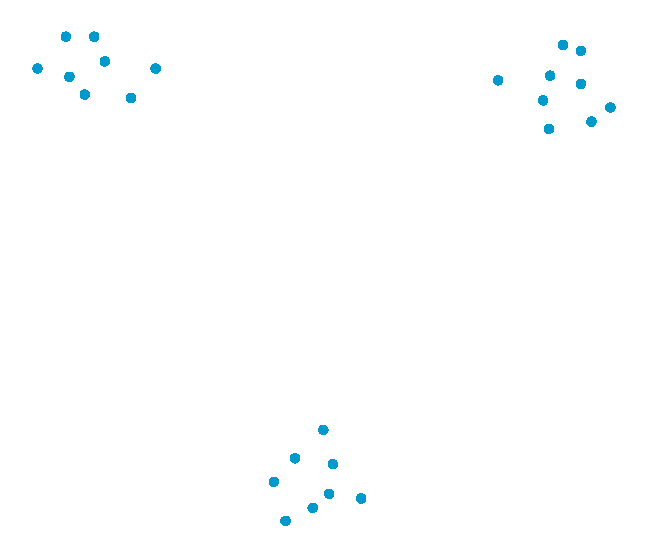
\includegraphics[width=.4\linewidth]{gfx/three_clusters_small.pdf}
    \caption{Dati divisi in più cluster}
    \label{fig:clusters}
  \end{center}
\end{figure}

Ad esempio, consideriamo un insieme di dati come in \cref{fig:clusters}. È chiaro a chi osserva che vi sono tre gruppi di punti, tuttavia la formalizzazione matematica di questa osservazione non è immediata.

Il modo usato dalla TDA è l'\emph{omologia persistente}, di cui diamo un'introduzione informale per poi riprenderlo in (NMDC: inserire riferimento al capitolo). Sia
\begin{equation*}
  X=\{x_1,\dots, x_n\}
\end{equation*}
il nostro insieme di dati. Consideriamo per $\varepsilon>0$ l'insieme
\begin{equation*}
  \widehat{X}_\varepsilon=\bigcup_{0\leq i\leq n} B(x_i,\varepsilon)
\end{equation*}
dove $B(x_i,\varepsilon)$ è la palla di centro $x_i$ e raggio $\varepsilon$. Osserviamo che esiste un intervallo di valori $a \leq \varepsilon \leq b$ per cui $\widehat{X}_\varepsilon$ appare come in \cref{fig:clusters_fat}.

\begin{figure}[h]
  \begin{center}
    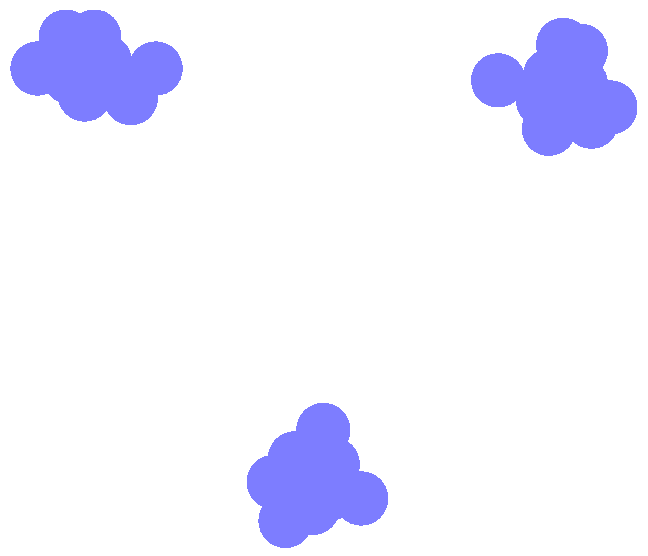
\includegraphics[width=.4\linewidth]{gfx/three_clusters_fat.pdf}
    \caption{$\widehat{X}_\varepsilon$}
    \label{fig:clusters_fat}
  \end{center}
\end{figure}

Allora possiamo possiamo calcolare il numero di componenti connesse di $\widehat{X}_\varepsilon$, o equivalentemente la dimensione del gruppo di omologia $H_{0}(\widehat{X}_\varepsilon;k)$, dove $k$ è un campo. L'osservazione che $X$ è composto essenzialmente da tre componenti è espressa dal fatto che
\begin{equation*}
  \mathrm{dim}_k(H_{0}(\widehat{X}_\varepsilon;k))=3
\end{equation*}
per un intervallo notevole di valori di $\varepsilon$, e da un certo $\overline{\varepsilon}$ in poi diventa~1.

Ovviamente, non è necessario parlare di dimensione del gruppo di omologia $H_{0}$ per discutere del numero di componenti connesse. Tuttavia, se consideriamo l'insieme di dati $X$ come in \cref{fig:circle}, possiamo chiederci come formalizzare l'intuizione che essi sono disposti in forma circolare.

\begin{figure}[h]
  \begin{center}
    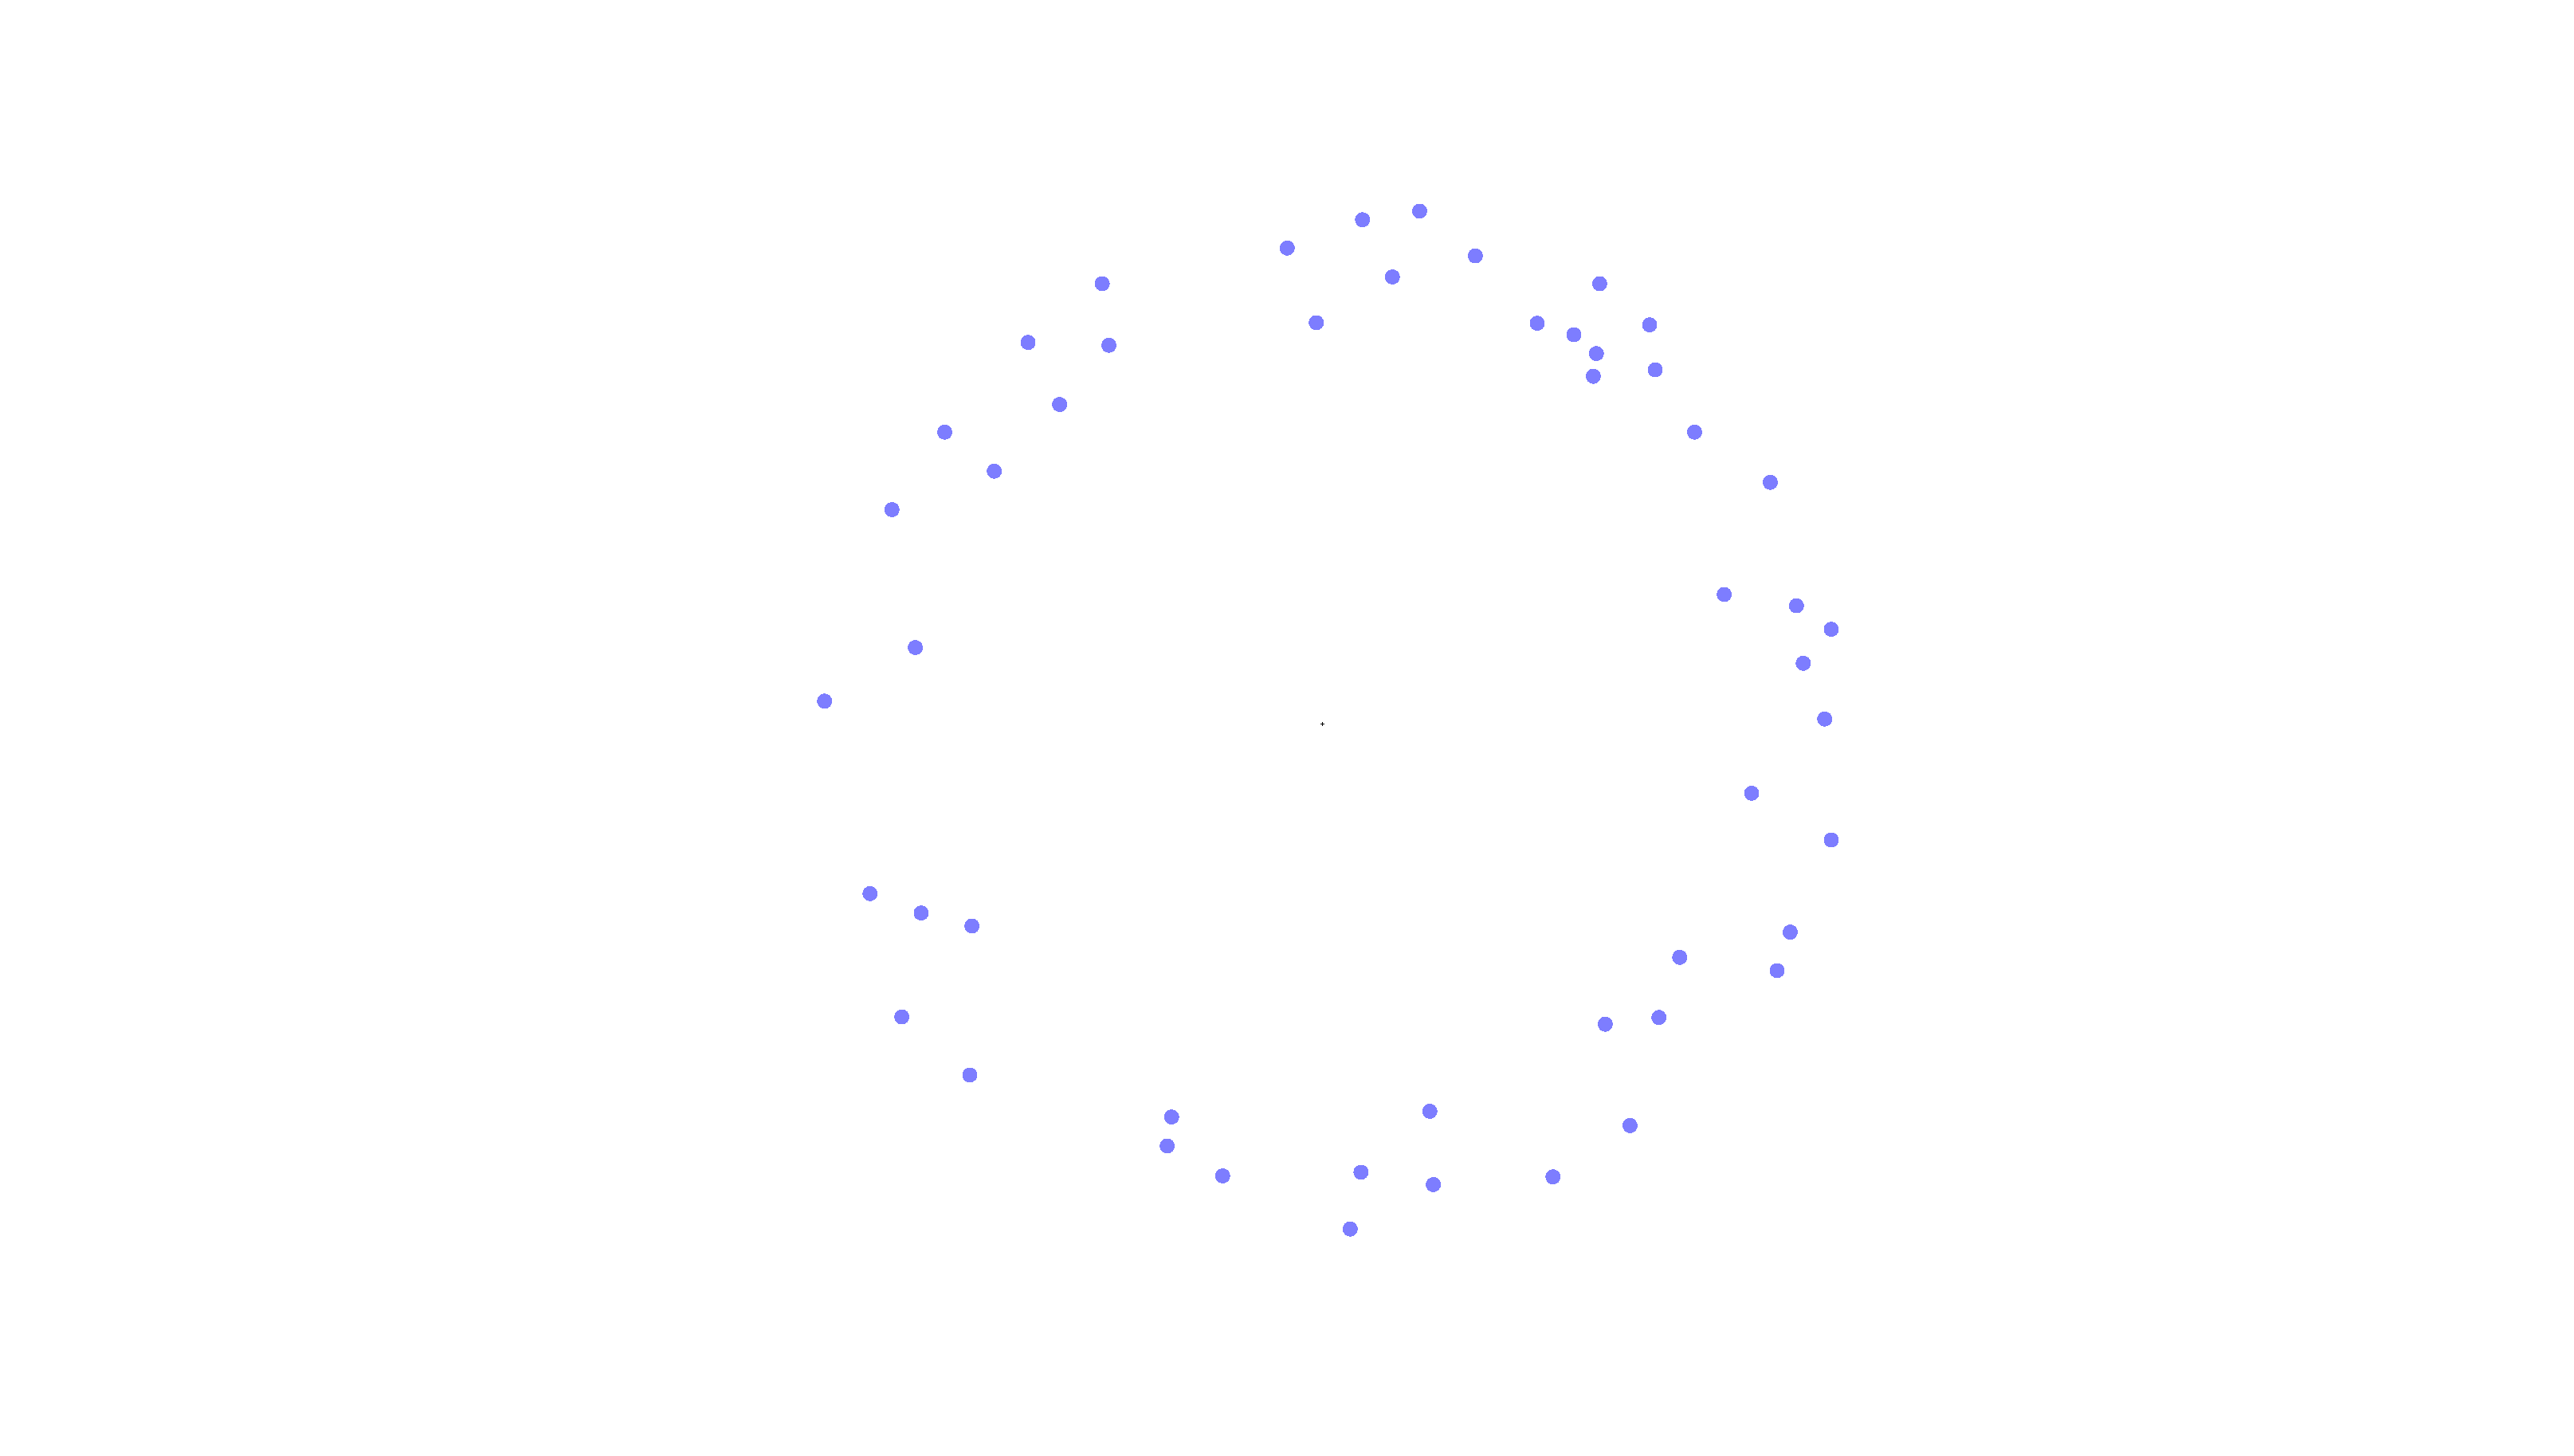
\includegraphics[width=\linewidth]{gfx/statistical_circle.pdf}
    \caption{Campionamento da una corona circolare}
    \label{fig:circle}
  \end{center}
\end{figure}

Ancora una volta possiamo considerare l'insieme $\widehat{X}_\varepsilon$ per diversi valori di $\varepsilon$ come in \cref{fig:circlecomparison} e considerare stavolta il gruppo di omologia $H_{1}(\widehat{X}_\varepsilon;k)$.

\begin{figure}[h]
  \begin{center}
    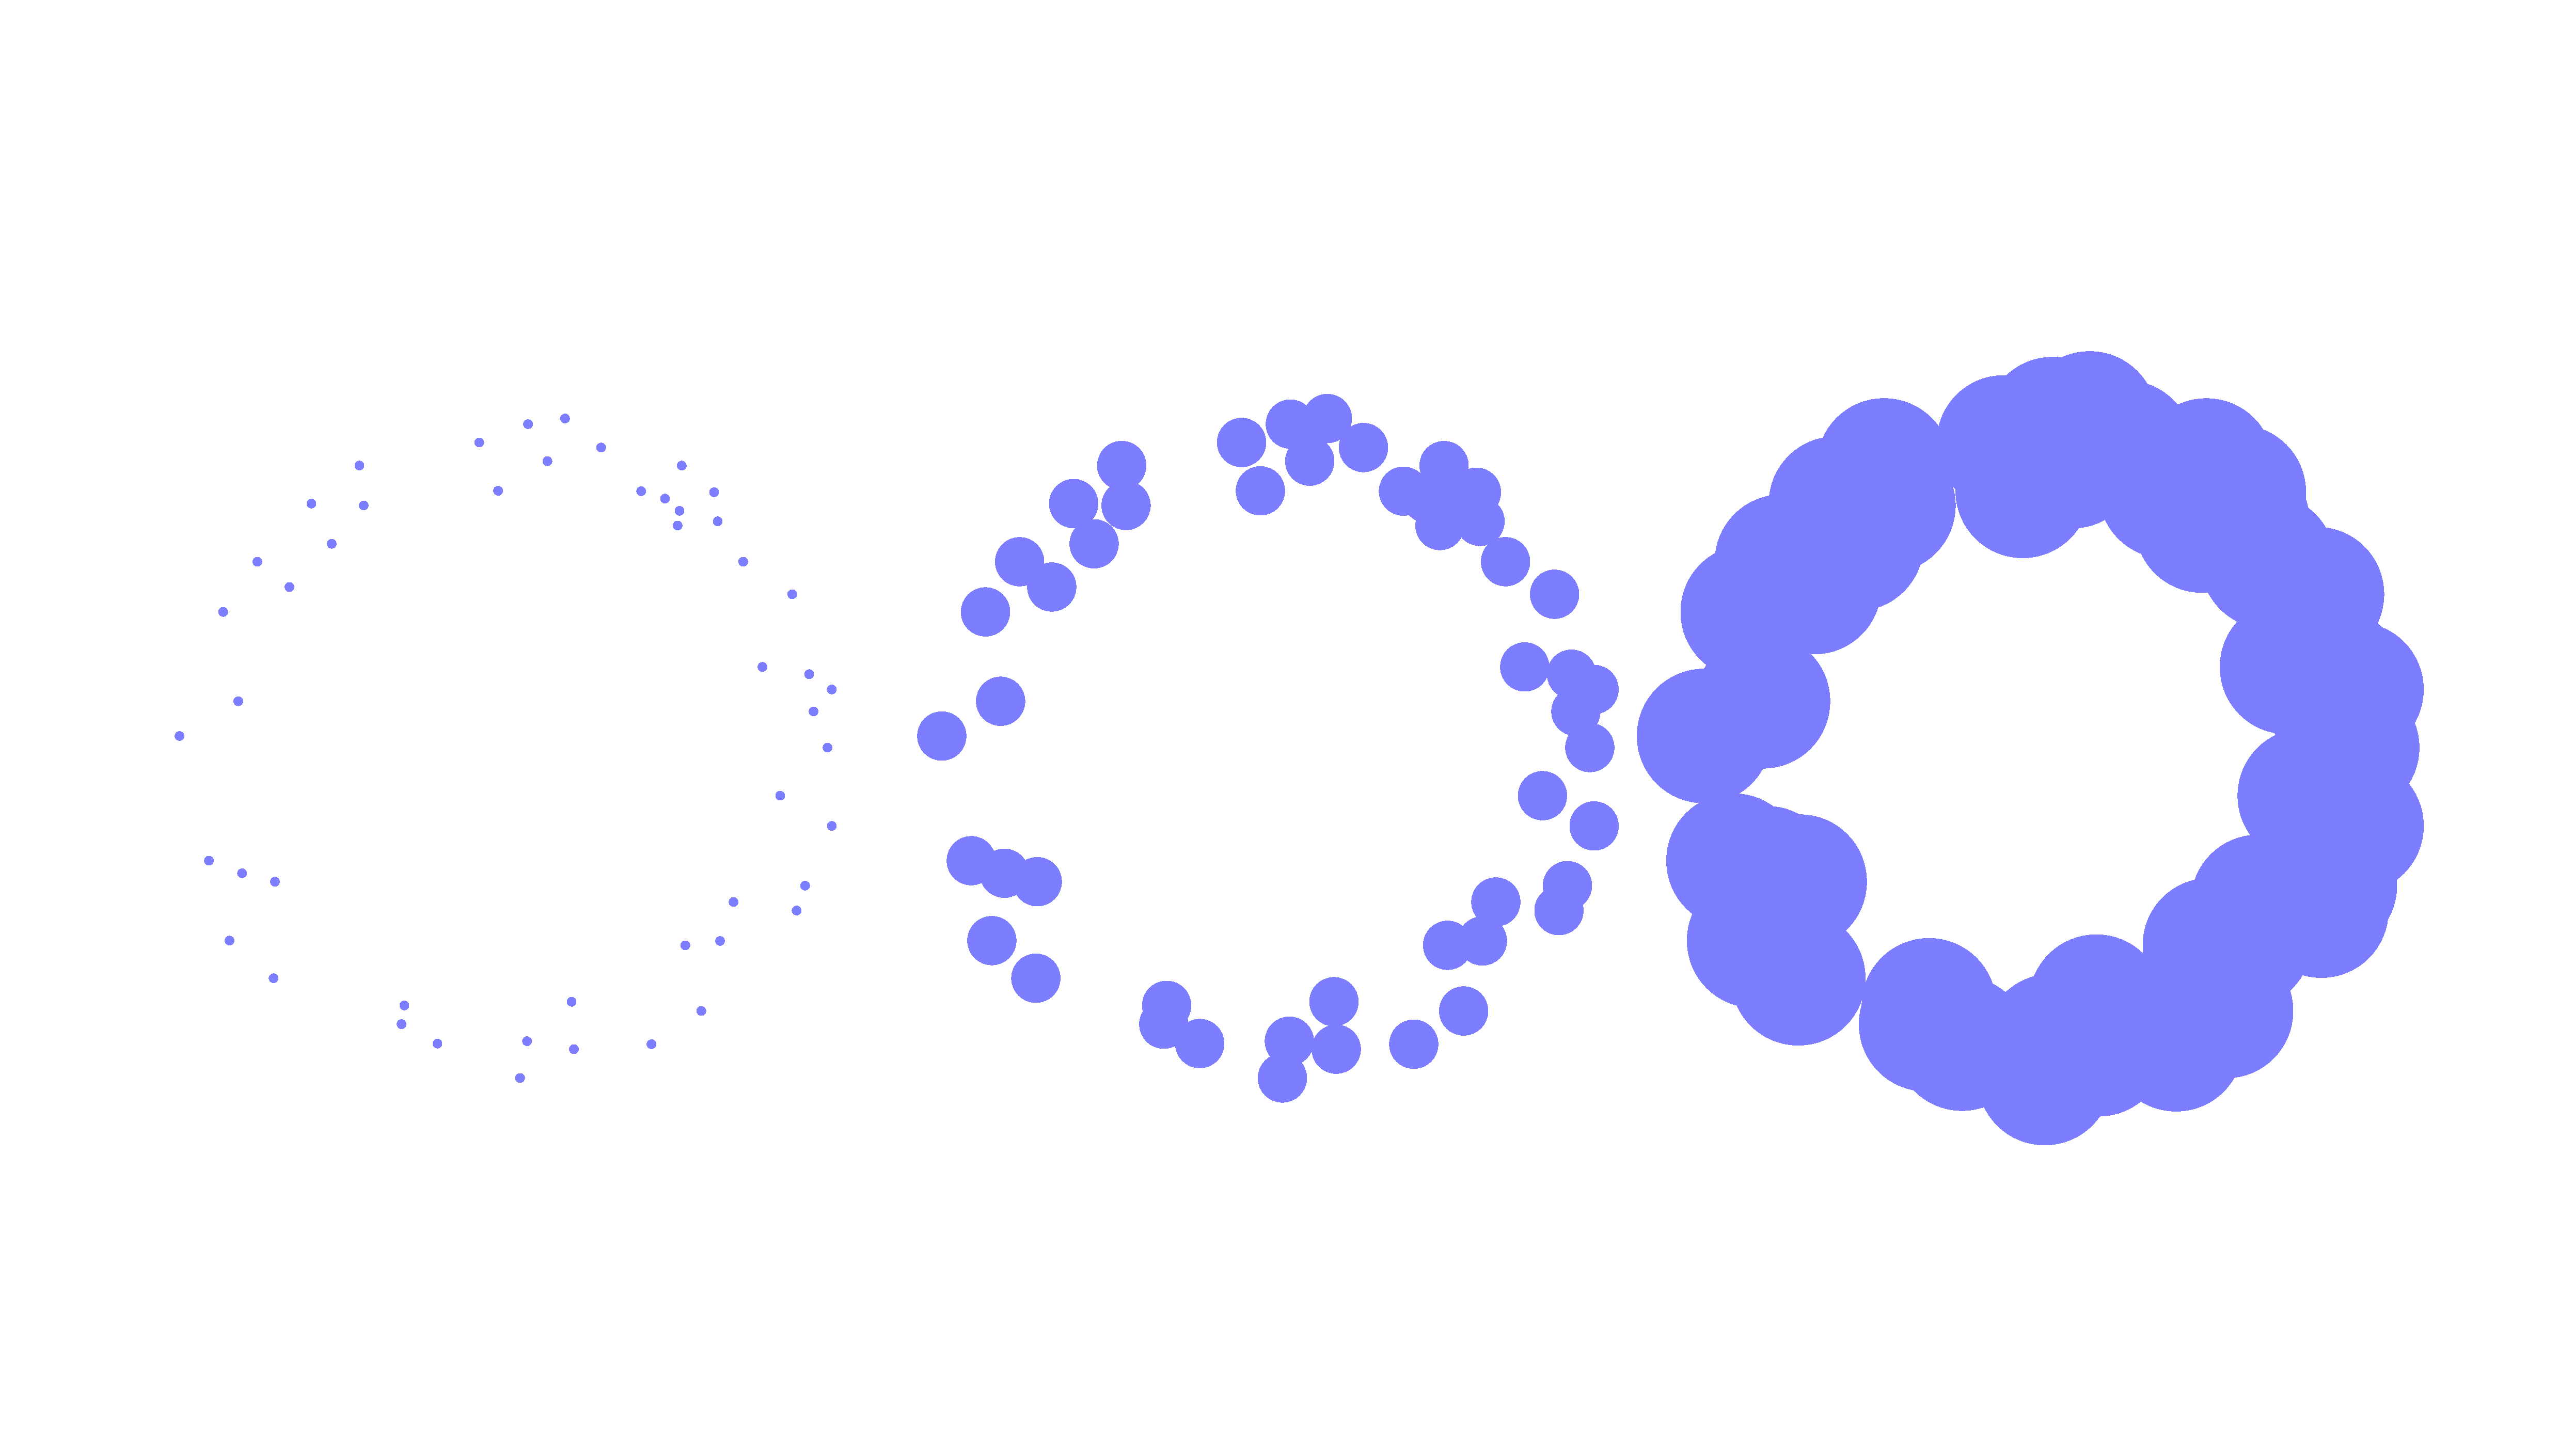
\includegraphics[width=.7\paperwidth]{gfx/statistical_circle_comparison.pdf}
    \caption{$\widehat{X}_\varepsilon$ al variare di $\varepsilon$}
    \label{fig:circlecomparison}
  \end{center}
\end{figure}

La dimensione di $H_1(\widehat{X}_\varepsilon;k)$ varia fino a stabilizzarsi su 1. Questo ci dice che c'è essenzialmente un buco 1-dimensionale nei dati.

Possiamo anche osservare variazioni di struttura al variare della scala di riferimento. Ad esempio, in \cref{fig:moreclusters} possiamo vedere che i tre cluster sulla sinistra collassano in un unico cluster se condiseriamo $\widehat{X}_\varepsilon$ per $\varepsilon \gtrsim e_2/2$.

\begin{figure}[h]
  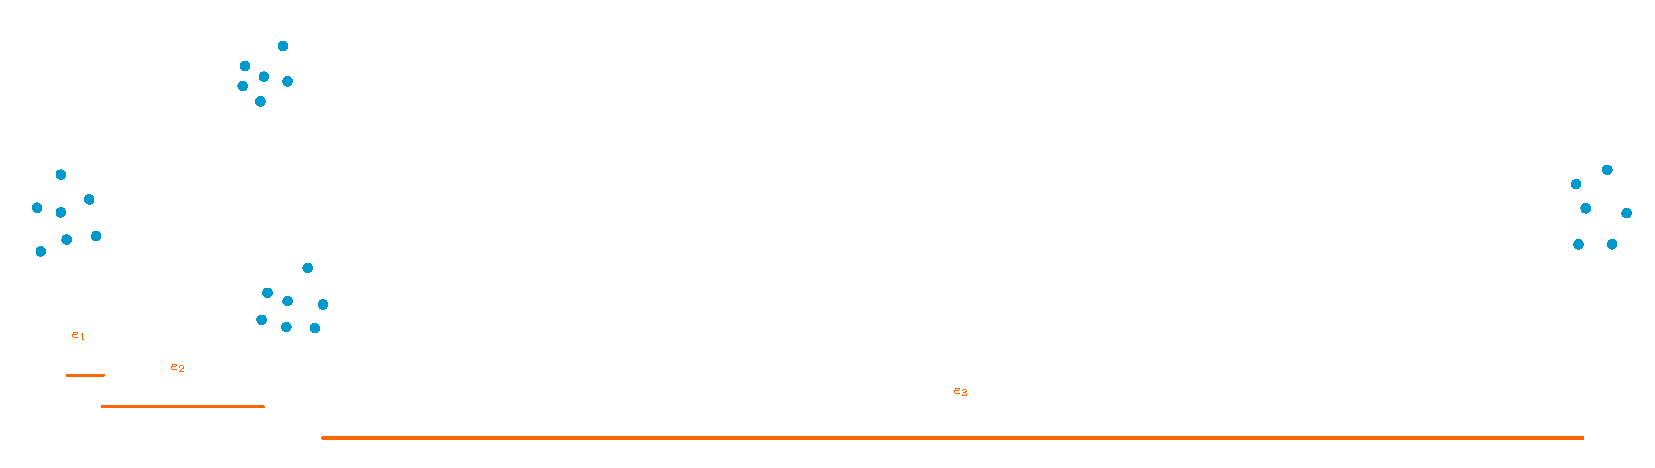
\includegraphics[width=.7\paperwidth]{gfx/more_clusters.pdf}
  \caption{Cluster su scale diverse}
  \label{fig:moreclusters}
\end{figure}

Per visualizzare l'andamento di $dim_k(\widehat{X}_\varepsilon)$ al variare di $\varepsilon$ usiamo un tipo di grafico chiamato \emph{persistence barcode}: per ogni \emph{feature} presente nei dati, disegnamo un segmento orizzontale lungo quanto l'intervallo di lunghezze di $\varepsilon$ in cui la feature persiste, come in \cref{fig:moreclusterbarcode}.

\begin{figure}[h]
  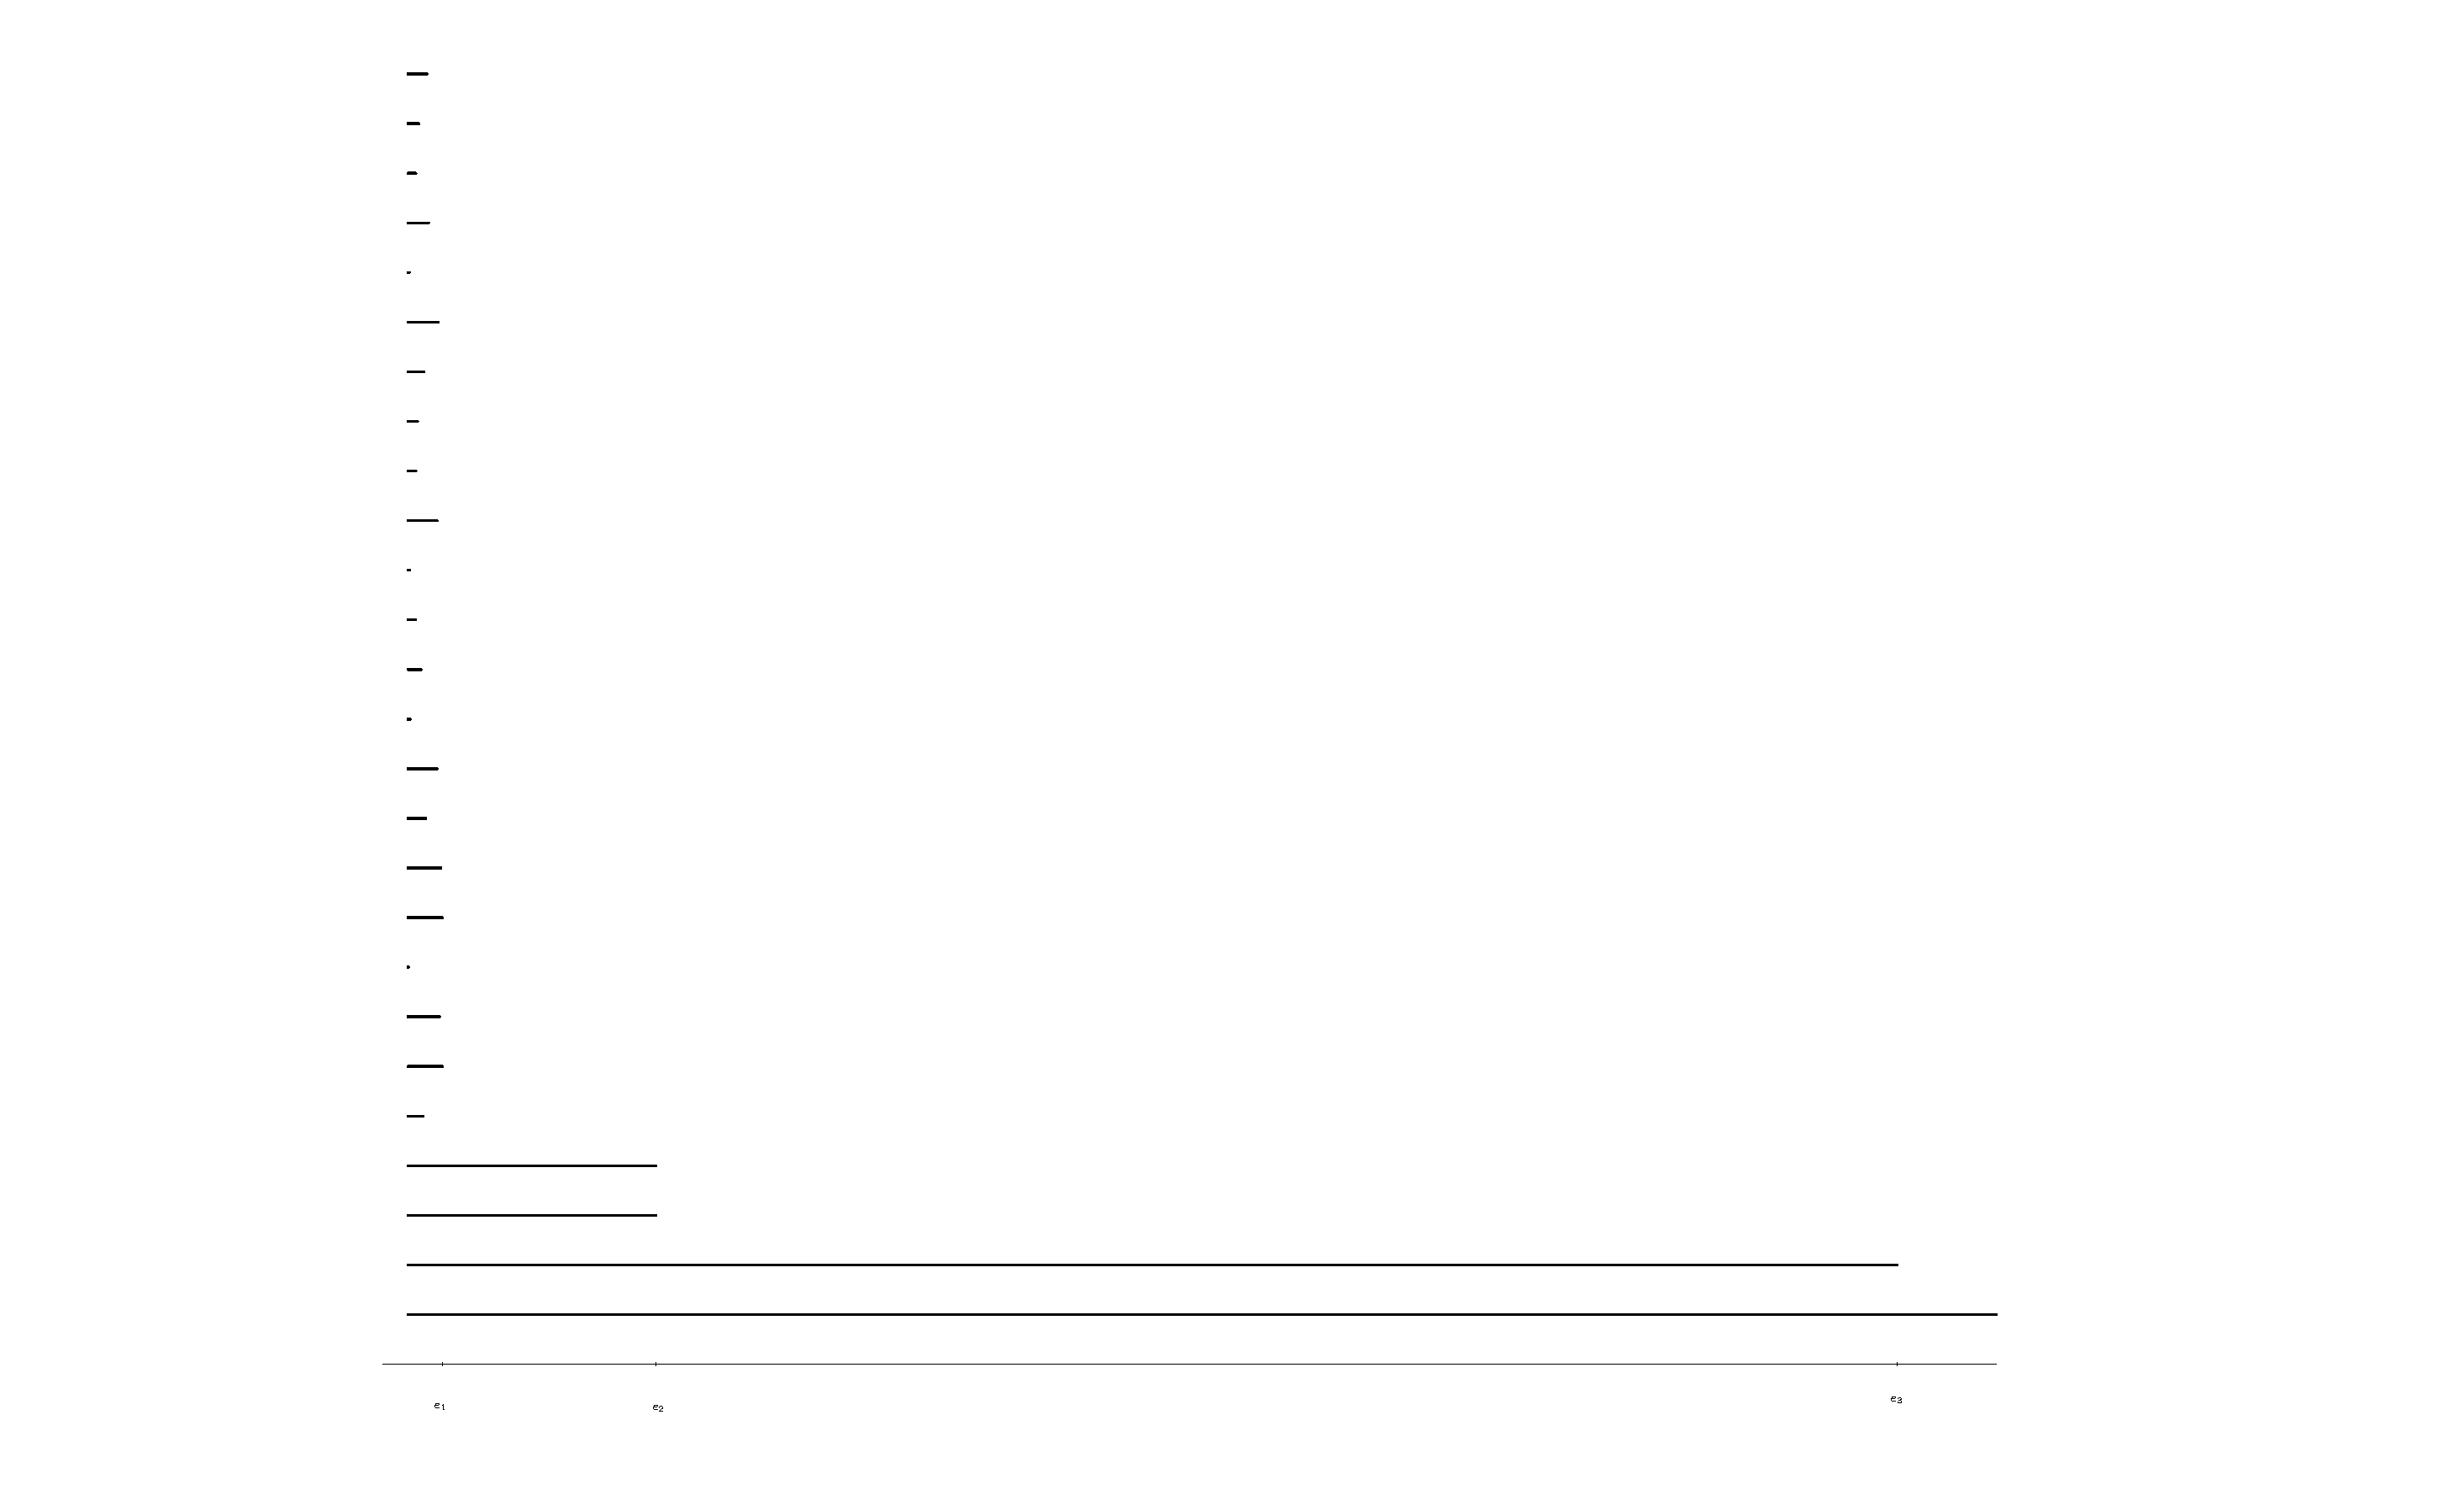
\includegraphics[width=.7\paperwidth]{gfx/more_clusters_barcodes.pdf}
  \caption{Un esempio di persistence barcode}
  \label{fig:moreclusterbarcode}
\end{figure}

Il grafico fa interpretato nel seguente modo: all'inizio vi sono 26 punti distinti, al crescere di $\varepsilon$ questi punti vengono uniti ad altri e quindi il numero si riduce, finché per $\varepsilon \gtrsim e_1/2$ restano essenzialmente 4 cluster, da $e_2/2$ ne restano solo due e da $e_3/2$ il gruppo di omologia $H_0(\widehat{X}_\varepsilon;k)$ diventa banale. (NMDC: aggiusta il grafico del barcode)

Possiamo sempre usare questa rappresentazione grazie alla decomposizione dei persistence barcodes garantita dal teorema (NMDC: aggiungere riferimento).

Un altro aspetto che l'omologia persistente cattura è la relazione fra i gruppi di omologia nelle diverse scale, in particolare $H_*(\widehat{X}_\varepsilon;k)$ è funtoriale rispetto all'ordine di $(\R,\leq)$, cioé se $\varepsilon_1 \leq \varepsilon_2$ allora c'è una mappa $H_*(\widehat{X}_{\varepsilon_1};k)\to H_*(\widehat{X}_{\varepsilon_2};k)$ e se $\varepsilon_1\leq\varepsilon_2\leq\varepsilon_3$, allora la mappa associata a $\varepsilon_1\leq\varepsilon_3$ è uguale alla composizione delle due mappe associate a $\varepsilon_1\leq\varepsilon_2$ e $\varepsilon_2\leq\varepsilon_3$.

Questo ci consente di catturare proprietà come quelle che si osservano in \cref{fig:doublecircle}.

\begin{figure}[ht]
  \begin{center}
    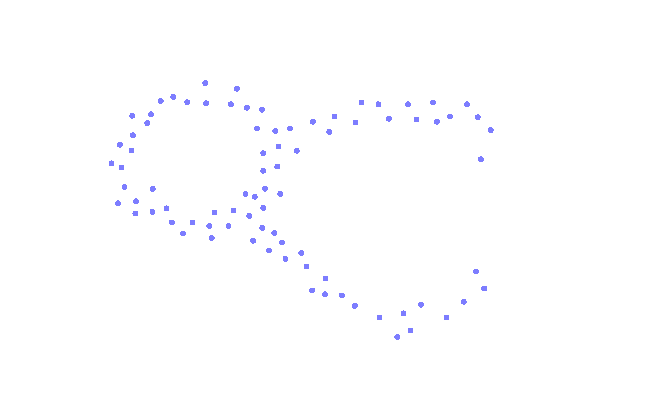
\includegraphics{gfx/double_circle_small.pdf}
    \caption{Un doppio anello}
    \label{fig:doublecircle}
  \end{center}
\end{figure}

In \cref{fig:doublecirclecomparison} osserviamo che al variare di $\varepsilon$ la dimensione di $H_1(\widehat{X}_\varepsilon;k)$ resta 1, tuttavia è chiaro che i due anelli sono due proprietà distinte dei dati. Questa distinzione non è racchiusa nel gruppo di omologia $H_1$, mentre la si vede dal fatto che la mappa
\begin{equation*}
H_1(\widehat{X}_{\varepsilon_1};k)\xto{0}H_1(\widehat{X}_{\varepsilon_2};k)
\end{equation*}
associata a $\varepsilon_1\leq\varepsilon_2$ è il morfismo nullo. Questo ci dice che non ci sono relazioni fra i due gruppi di omologia.

\begin{figure}[ht]
  \begin{center}
    \begin{subfigure}[b]{.4\textwidth}
      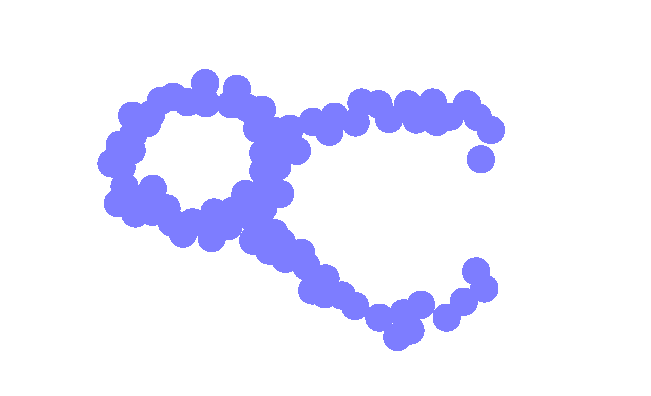
\includegraphics[width=\textwidth]{gfx/double_circle_medium.pdf}
      \caption{$\widehat{X}_{\varepsilon_1}$}
    \end{subfigure}
    \begin{subfigure}[b]{.4\textwidth}
      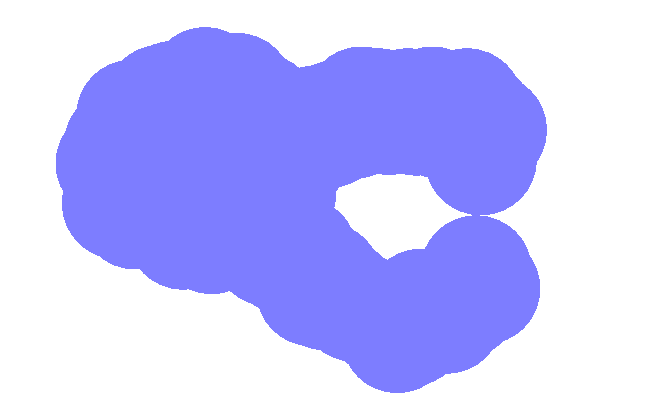
\includegraphics[width=\textwidth]{gfx/double_circle_fat.pdf}
      \caption{$\widehat{X}_{\varepsilon_2}$}
    \end{subfigure}
    \caption{Variazione delle proprietà di $\widehat{X}_\varepsilon$}  \label{fig:doublecirclecomparison}
  \end{center}
\end{figure}

(NMDC:dire qualcosa sull'algoritmo Mapper?)

Nel resto del capitolo ci occuperemo di costruire l'omologia persistente, con attenzione all'aspetto computazionale.

\clearpage

\section{Omologia simpliciale}

\begin{sloppypar}
  Fissato un campo $k$, ad ogni spazio topologico possiamo associare una successione di $k$-spazi vettoriali $H_i(X;k)$ detti \emph{gruppi di omologia}. Per la precisione si tratta di una successione di funtori ${H_*(-;k):\Top \to \Vectk}$. Nel resto della sezione ci occuperemo di definire in modo operativo questi gruppi.
\end{sloppypar}

Esistono diversi modi di calcolare i gruppi di omologia. Il più generale e potente è l'omologia singolare, tuttavia questa risulta scomoda da usare in pratica perché richiede di lavorare con quozienti di spazi vettoriali di dimensione più che numerabile. Per aggirare il problema definiremo soltanto l'omologia simpliciale.

In virtù degli assiomi di Eilenberg-Steenrod \cite{Eilenberg1945, Eilenberg} le due definizioni sono equivalenti (almeno per gli spazi che andremo a considerare). Per una trattazione più dettagliata si vedano \cite{Hatcher2015} o \cite{Rotman1988}.

Si procederà associando all'insieme di dati $X$ uno spazio topologico (detto complesso simpliciale) per ogni parametro $\varepsilon \in \R^+$ e si definirà l'omologia solo per questi particolari spazi topologici.

Gli spazi $\widehat{X}_\varepsilon$ usati nell'introduzione, sebbene comodi per introdurre un'idea intuitiva di persistenza, non sono l'ambiente naturale in cui lavorare, quindi non verranno più usati nella trattazione formale. Si osservi, però, che l'omologia di $\widehat{X}_\varepsilon$ è equivalente all'omologia del complesso simpliciale di \v{C}ech di parametro $\varepsilon$ associato a $X$. Per questioni di comodità, tuttavia, noi lavoreremo principalmente con il complesso di Vietoris-Rips.

\subsection{Complessi simpliciali}

\begin{sloppypar}
  I complessi simpliciali sono particolari spazi topologici che hanno una descrizione combinatorica. Dato un insieme di punti ${S=\{s_0,\dots,s_n\}}$ in $\R^k$ diremo che sono in posizione generale se non sono contenuti in nessun sottospazio affine di dimensione minore di $n$. Se $S$ è in posizione generale, il suo inviluppo convesso $\sigma(S)$ è detto \emph{($n$-)simplesso generato da $S$}. I punti $s_i$ di $S$ si chiamano \emph{vertici} di $\sigma(S)$. Se $\emptyset\neq T$ è un sottinsieme di $S$, $\sigma(T)$ è detto \emph{faccia} di $\sigma(S)$.
\end{sloppypar}

Con questi ingredienti possiamo dare la seguente
\begin{definition}
Un \emph{complesso simpliciale} (finito) $K$ è una famiglia finita di simplessi in uno spazio euclideo tali che:
\begin{enumerate}
  \item Se $\sigma\in K$ e $\tau$ è una faccia di $\sigma$, allora $\tau \in K$.
  \item Se $\sigma,\tau\in K$, allora il simplesso $\sigma\cap\tau$ è una faccia sia di $\sigma$ sia di $\tau$.
\end{enumerate}
\end{definition}

\`E chiaro che un complesso simpliciale è determinato essenzialmente da proprietà combinatoriche dell'insieme dei suoi vertici, che motiva la seguente costruzione astratta.

\begin{definition}
  Un \emph{complesso simpliciale astratto} $X$ è il dato della coppia $(V(X), \Sigma(X))$, dove $V(X)$ è un insieme finito, i cui elementi sono i \emph{vertici} di $X$, e $\Sigma(X)$ è una famiglia di sottinsiemi non vuoti di $V(X)$, i cui elementi sono detti \emph{simplessi} di $X$, tale che:
  \begin{enumerate}
    \item se $v\in V(X)$ allora $\{v\}\in\Sigma(X)$, e
    \item se $\sigma \in \Sigma(X)$ e $\emptyset\neq\tau\subseteq\sigma$, allora $\tau\in\Sigma(X)$.
  \end{enumerate}

  Un simplesso $\sigma\in\Sigma(X)$ è detto $q$-simplesso se $|\#\sigma| = q+1$. Indichiamo con $X_q$ l'insieme dei $q$-simplessi di $X$.
\end{definition}

\begin{rmk}
  Ogni complesso simpliciale $K$ determina un complesso simpliciale astratto $\widehat{K}$ tale che $V(\widehat{K})$ è l'insieme dei vertici dei simplessi di $K$ e un sottinsieme di $V(\widehat{K})$ è in $\Sigma(\widehat{K})$ se e solo se è l'insieme dei vertici di un simplesso di $K$.
\end{rmk}

Possiamo anche definire i morfismi $f:X\to Y$ fra complessi simpliciali astratti come le mappe $f_V:V(X)\to V(Y)$ fra i sottostanti insiemi di vertici e tali che $f_V(\sigma)\in \Sigma(Y)$ per ogni $\sigma \in \Sigma(X)$.

(NMDC: inserire qualche disegno, eventualmente un riferimento a qualche testo sugli oggetti simpliciali)

Ad ogni complesso simpliciale astratto $X$ si può associare un complesso simpliciale $|X|$ detto la \emph{realizzazione geometrica} di $X$ (NMDC: aggiungere un riferimento) e tale che i morfismi $f:X\to Y$ siano mandati in mappe continue $|f|:|X|\to |Y|$ in maniera funtoriale, cioé $|g\circ f|=|g|\circ |f|$. Inoltre, ogni complesso simpliciale $K$ è omeomorfo alla realizzazione geometrica del complesso simpliciale astratto $\widehat{K}$ ad esso associato.

\subsection{Omologia simpliciale}

Ora definiremo i gruppi di omologia associati a un complesso simpliciale astratto.

\begin{definition}
  Sia $k$ un gruppo o un campo o un anello e
  sia $X=(V(X),\Sigma(X))$ un complesso simpliciale astratto, insieme con un ordine totale sull'insieme $V(X)$. Il gruppo dei \emph{$q$-cicli} di $X$ su $k$ è il $k$-modulo $C_q(X,k)$ generato dagli elementi
  \begin{itemize}
    \item $[v_0,\dots, v_q]$ con $v_0,\dots, v_q\in V(X)$ e tali che $\{v_0,\dots,v_q\}\in\Sigma(X)$
  \end{itemize}
  modulo le seguenti relazioni:
  \begin{enumerate}
    \item $[v_0,\dots,v_q]=0$ se $v_i = v_j$ per qualche $i\neq j$,
    \item $[v_{\sigma(0)},\dots,v_{\sigma(q)}]=sign(\sigma)[v_0,\dots,v_q]$ per ogni permutazione $\sigma$ di $\{0,\dots,q\}$.
  \end{enumerate}

  Scriveremo $C_*(X,k)$ per indicare tutti i gruppi dei cicli in tutti i gradi, eventualmente sottintendendo il campo $k$.
\end{definition}

\begin{rmk}
  Nella definizione precedente si è tenuta traccia dell'ordine dei vertici dei complessi simpliciali perché esso è importante ai fini dell'omologia, dunque d'ora in poi consideriamo sempre i complessi simpliciali ordinati.
\end{rmk}

\begin{lemma}\label{lemma:sollcicli}
  Dati due complessi simpliciali astratti $X$ e $Y$ e un morfismo $f$ fra essi, allora $f$ induce un omomorfismo $f_q:C_q(X)\to C_q(Y)$ per ogni $q\in\N$ definito da:
  \begin{align*}
    f_q:C_q(X)\longrightarrow & C_q(Y)\\
    [v_0,\dots,v_q] \mapsto & [f(v_0),\dots,f(v_q)].
  \end{align*}

  Scriveremo $f_*:C_*(X)\to C_*(Y)$ per indicare tutti questi morfismi.
\end{lemma}

\begin{rmk}
  Il motivo per cui il gruppo dei $q$-cicli è stato introdotto mediante generatori e relazioni è che in questo modo è più facile sollevare mappe di complessi simpliciali astratti a omomorfismi fra i gruppi dei cicli. Se avessimo semplicemente definito il gruppo dei $q$-cicli come il $k$-modulo generato da $X_q$ sarebbe stato necessario modificare la definizione di $f_*$ in modo che i cicli mappassero correttamente, perdendo notevolmente in eleganza.
\end{rmk}

\begin{definition}
  Sia $X$ un complesso simpliciale astratto, allora esistono morfismi $\partial^X_q:C_q(X) \to C_{q-1}(X)$ per ogni $q\in\N_0$ definiti come:
  \begin{equation*}
    \partial_q([v_0,\dots,v_q])=\sum_{i=0}^q (-1)^i[v_0,\dots,\widehat{v}_i,\dots,v_q]
  \end{equation*}
  dove la notazione $\widehat{v}_i$ significa che l'$i$-mo elemento non è presente. Scriveremo $\partial$ invece che $\partial^X$ quando non è necessario specificare il complesso simpliciale sottostante.
\end{definition}

\begin{lemma}
  Nelle notazioni precedenti, $\partial_{q-1}\circ \partial_q=0$.
\end{lemma}

\begin{rmk}
  Il lemma precedente ci dice che per ogni complesso simpliciale astratto $X$ i suoi cicli $C_*(X)$ formano un complesso di $k$-moduli. Allora data una mappa di complessi simpliciali astratti $f:X\to Y$, il suo sollevamento $f_*:C_*(X)\to C_*(Y)$ è un morfismo di complessi di $k$-moduli, cioé $f_{q-1}\circ \partial^X_q=\partial^Y_q\circ f_q$. Quest'ultima proprietà può essere espressa dicendo che il seguente diagramma è commutativo (cioé che qualsiasi percorso si segua componendo i morfismi non cambia il risultato della composizione).
  \begin{equation*}
    \begin{tikzcd}
      C_q(X)\arrow[r,"\partial^X_q"]\arrow[d,"f_q"]
        &C_{q-1}(X)\arrow[d,"f_{q-1}"]\\
      C_q(Y)\arrow[r,"\partial^Y_q"]&C_{q-1}(Y)
    \end{tikzcd}
  \end{equation*}

  Possiamo visualizzare $C_*(X)$ come la seguente successione:
  \begin{equation*}
    \begin{tikzcd}
      \dots \arrow{r}&
        C_2\arrow{r}{\partial_2}&
          C_1\arrow{r}{\partial_1}&
            C_0
    \end{tikzcd}
  \end{equation*}
  a cui per completezza aggiungeremo il morfismo $\partial_0:C_0\to 0$.
\end{rmk}

\begin{definition}
  Dato un complesso impliciale astratto $X$, per ogni $q\in\N_0$ vale $Im\,\partial_q \subseteq Ker\,\partial_{q-1}$. Definiamo il $q$-mo gruppo di omologia di $X$ come il quoziente
  \begin{equation*}
    H_q(X) = \frac{Ker\,\partial_q}{Im\,\partial_{q+1}}.
  \end{equation*}
\end{definition}

Il seguente esempio serve a mostrare intuitivamente come l'omologia è collegata alle proprietà geometriche di un complesso simpliciale. Consideriamo il complesso simpliciale astratto $X=(V(X),\Sigma(X))$ con:
\begin{align*}
  V(X) &= ( A,B,C,D,E )\\
  \Sigma(X) &= \{ \{A\}, \{B\}, \{C\}, \{D\}, \{E\}, \{A,B\}, \{C,D\}, \{D,E\}, \{C,E\} \}
\end{align*}
rappresentato in figura \cref{fig:simplicialcomplex}. La scrittura $(A,\dots,E)$ indica che l'ordine è $A<\dots<E$.

\begin{figure}[h]
  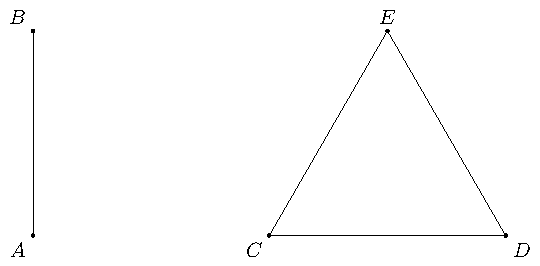
\includegraphics[width=.7\linewidth]{gfx/example_homology.pdf}
  \caption{Un complesso simpliciale}
  \label{fig:simplicialcomplex}
\end{figure}

Allora $C_0$ è lo spazio vettoriale generato da $[A], [B], [C], [D], [E]$ e $C_1$ da $[A,B], [C,D], [D,E], [C,E]$.
Applicando il differenziale $\partial_1$ ai generatori di $C_1$ otteniamo:
\begin{align*}
  \partial_1([A,B]) &= [B] - [A]\\
  \partial_1([C,D]) &= [D] - [C]\\
  \partial_1([D,E]) &= [E] - [D]\\
  \partial_1([C,E]) &= [E] - [C]
\end{align*}

Per semplicità, si può anche scrivere $\partial_1$ in forma matriciale come
\begin{equation*}
  \bordermatrix{
     & [A,B] & [C,D] & [D,E] & [C,E]\cr
    [A] & -1 & 0 & 0 & 0 \cr
    [B] & 1 & 0 & 0 & 0 \cr
    [C] & 0 & -1 & 0 & -1 \cr
    [D] & 0 & 1 & -1 & 0\cr
    [E] & 0 & 0 & 1 & 1\cr
  },
\end{equation*}
da cui risulta evidente che $Im\,\partial_1$ ha dimensione 3, quindi $H_0(X) = Ker\,\partial_0 / Im\,\partial_1$ è un $k$-spazio di dimensione $2$. Si osservi che $X$ ha esattamente 2 componenti connesse.

Analogamente $Ker\,\partial_1$ ha dimensione 1 e $C_2$ è lo spazio banale, quindi $H_1(X)$ ha dimensione 1, che rappresenta il fatto che c'è un loop nella spezzata $[C,D] + [D,E] + [E,C]$ (infatti $Ker\,\partial_1$ è generato proprio da questo vettore).

\begin{figure}[h]
  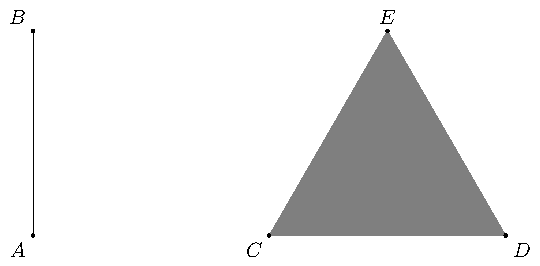
\includegraphics[width=.7\linewidth]{gfx/example_homology_loop.pdf}
  \caption{Il complesso $X$ con l'aggiunta di un $2$-simplesso}
  \label{fig:simplicialcomplexloop}
\end{figure}

Se aggiungiamo a $X$ il simplesso $\{C,D,E\}$ come in \cref{fig:simplicialcomplexloop} abbiamo che $C_2$ è generato da $[C,D,E]$ e $\partial_2([C,D,E]) = [D,E] - [C,E] + [C,D] = [C,D] + [D,E] + [E,C]$. Quindi chiudendo il loop con un simplesso abbiamo che
$Im\,\partial_2 = Ker\,\partial_1$ e $H_1(X)$ è lo spazio banale.

\begin{rmk}
  L'assegnazione di $H_*(X)$ a un complesso simpliciale astratto $X$ è in realtà un funtore, cioé per ogni morfismo di complessi simpliciali astratti $f:X\to Y$ esiste un omomorfismo di $k$-spazi vettoriali $f_*:H_*(X)\to H_*(Y)$ (e in realtà $f_*$ è il morfismo indotto da $f_*:C_*(X)\to C_*(Y)$) e $(g\circ f)_* = g_* \circ f_*$.
\end{rmk}

\section{Omologia Persistente}\label{sec:persistenthomology}

Nella sezione precedente è stata definita l'omologia simpliciale e si è visto con alcuni esempi come questa sia collegata a proprietà topologiche del complesso simpliciale in analisi. Quello che resta per poter usare l'omologia per studiare una nube di punti è un modo di costruire un simplesso simpliciale a partire dai dati, il che essenzialmente si riduce a studiare i dati ad una certa scala di grandezza. Tuttavia, non è necessariamente ovvio come fare e, come si è visto nell'introduzione, talvolta non esiste una scelta di scala che consenta di catturare tutte le proprietà (omologiche) dei nostri dati.

Per questo motivo si introduce il concetto di persistenza, che è un modo di controllare diverse scale contemporaneamente e le relazioni tra queste.

\begin{definition}\label{def:persistentset}
  Un \emph{insieme persistente} è una famiglia di insiemi $\{X_r\}_{\R}$ indicizzata da $\R$ e tale che per ogni coppia di numeri reali $r<s$ esiste una funzione $f_{s,r}:X_r\to X_s$ e queste funzioni sono tali che se $r< s< t$ allora $f_{t,r} = f_{t,s}\circ f_{s,r}$. Più in generale un oggetto persistente in una categoria $\mathcal{C}$ è un funtore $(R,\leq)\to \mathcal{C}$, quindi si può parlare di \emph{spazi vettoriali persistenti},
  \emph{spazi topologici persistenti}, \emph{complessi simpliciali persistenti}, ecc.
\end{definition}

A questo punto è possibile associare un complesso simpliciale astratto ai nostri dati nel seguente modo.

\begin{definition}
  Sia $X$ uno spazio metrico finito. Fissato un numero reale positivo $r$ il \emph{complesso di Vietoris-Rips} di $X$ è
  un complesso simpliciale astratto $VR(X,r)$ così definito:
  \begin{itemize}
    \item l'insieme dei vertici di $VR(X,r)$ è $X$,
    \item la collezione $\{x_0,\dots,x_n\}\subseteq X$ è un simplesso di $VR(X,r)$ se e solo se
    \begin{equation*}
      d(x_i,x_j) \leq r \mathrm{\text{ per tutti gli }}i,j\in\{0,\dots,n\}.
    \end{equation*}
  \end{itemize}
\end{definition}

\begin{rmk}
  Se $r<s$ esiste un'ovvia iniezione $VR(X,r)\to VR(X,s)$, siccome gli insiemi dei vertici coincidono e ogni simplesso di $VR(X,r)$ è anche un simplesso di $VR(X,s)$, quindi la famiglia $\{VR(X,r)\}_{r\in\R}$ forma un complesso simpliciale persistente.
\end{rmk}

\begin{figure}[h]
  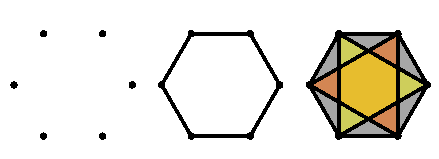
\includegraphics[width=.7\linewidth]{gfx/exhagon.pdf}
  \caption{Esempio di complesso di Vietoris-Rips}
  \label{fig:exhagon}
\end{figure}

Ad esempio si consideri un esagono regolare come in \cref{fig:exhagon}. Se $R$ è la misura del lato dell'esagono, le tre figure rappresentano $VR(X,r)$ rispettivamente con $0\leq r < R$, $R\leq r < \sqrt{3}R$, e $r \geq \sqrt{3}R$. I complessi di Vietoris-Rips sono elementari nelle prime due figure. Si osservi, invece, che nella terza vi sono 8 $2$-simplessi, sebbene intuitivamente sia sufficiente usarne 4 per vedere che lo spazio diventa banale a quella scala.

\begin{sloppypar}
  A questo punto applicando $H_*(-,k)$ a $\{VR(X,r)\}_{\R}$ otteniamo una famiglia di spazi vettoriali $\{H_*(VR(X,r),k)\}$ che insieme alle mappe ${H_*(f_{s,r},k):H_*(VR(X,r))\to H_*(VR(X,s))}$ formano uno spazio vettoriale persistente. Osserviamo inoltre che essendo partiti da uno spazio metrico finito $X$ ci saranno solo un numero finito di complessi di Vietoris-Rips al variare di $r$.
\end{sloppypar}

Gli spazi $\{H_*(VR(X,r),k)\}_{r\in\R}$ racchiudono l'informazione topologica dello spazio metrico $X$, tuttavia questa definizione astratta potrebbero sembrare di difficile utilizzo: assumendo di poter calcolare tutti gli $H_q(VR(X,r),k)$ per tutti gli $r$ e per piccoli valori di $q$, la domanda successiva diventa cosa si può dire delle interazioni fra i vari complessi su scale diverse?

\begin{sloppypar}
  In linea di principio dobbiamo considerare per ogni ${f_{s,r}:VR(X,r)\to VR(X,s)}$ non banale l'associato morfismo di spazi vettoriali ${H_q(f_{s,r}):H_q(VR(X,r))\to H_q(VR(X,s))}$ e tenere traccia delle dimensioni degli spazi $H_q(VR(X,r))$, $H_q(VR(X,s))$, e $Im\,H_q(f_{s,r})$.
\end{sloppypar}

Al fine di poter meglio comprendere come sono fatti i gruppi di omologia persistenti, studiamo meglio gli spazi vettoriali persistenti. D'ora in poi per semplicità diremo che $V$ è uno spazio vettoriale persistente invece che indicare esplicitamente tutta la famiglia $\{V_r\}$. Qualora fosse necessario esplicitare i morfismi $f_{s,r}:V_r\to V_s$ li indicheremo con la notazione $(V,f)$.

\begin{definition}
  Sia $I\subseteq \R$. Diremo che $I$ è un intervallo di $\R$ se dati comunque $r,s\in I$ tali che $r<s$ e $t$ tale che $r<t<s$, allora anche $t\in I$. Definiamo \emph{moduli intervallo} gli spazi vettoriali persistenti $k_I$, dove $I$ è un intervallo di $\R$, tali che $k_I(r) = k$ se $r\in I$ e $0$ altrimenti.
\end{definition}

\begin{definition}
  Si definisce \emph{somma diretta} di due spazi vettoriali persistenti $(V,f^V)$ e $(W,f^W)$ lo spazio vettoriale persistente $U$ definito come $U_r = V_r\oplus W_r$ per ciascun $r$ e $f^U_{s,r} = f^V_{s,r}\oplus f^W_{s,r}$, e lo si indica come $(V\oplus W,f^V\oplus f^W)$.
\end{definition}

\begin{figure}[ht]
  \begin{center}
    \begin{subfigure}[b]{.4\textwidth}
      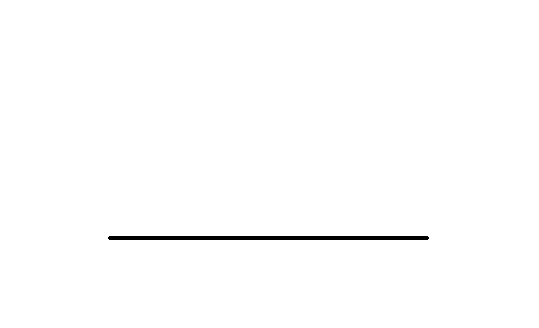
\includegraphics[width=\textwidth]{gfx/barcodes_single.pdf}
      \caption{$k_I$}\label{fig:barcodes:single}
    \end{subfigure}
    \begin{subfigure}[b]{.4\textwidth}
      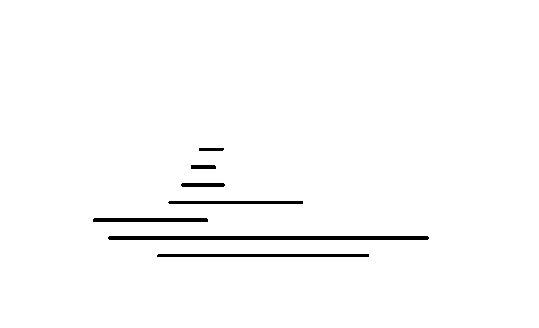
\includegraphics[width=\textwidth]{gfx/barcodes_multiple.pdf}
      \caption{$\bigoplus_{I\in\mathcal{D}} k_I$}\label{fig:barcodes:multiple}
    \end{subfigure}
    \caption{Esempi di codici a barre}  \label{fig:barcodes}
  \end{center}
\end{figure}


Poiché i moduli intervallo sono associati a intervalli di $\R$ li si può rappresentare come barre lunghe quanto l'intervallo ad essi associati (\cref{fig:barcodes:single}), e similmente una somma diretta finita di moduli intervallo
$k_{I_1}\oplus k_{I_2}\oplus\cdots \oplus k_{I_n}$ può essere rappresentata con quelli che sono detti codici a barre (\cref{fig:barcodes:multiple}). Il seguente teorema ci dice che in realtà tutti gli spazi vettoriali persistenti si posso rappresentare in questo modo.

\begin{theorem}[Decomposizione degli spazi vettoriali persistenti \cite{Crawley-Boevey2012}]\label{thm:persistentdecomposition}
  Sia $(V,f)$ uno spazio vettoriale persistente tale che $V_r$ ha dimensione finita per ogni $r\in\R$, allora esiste un
  multi-insieme $\mathcal{D}$ di intervalli, cioé una famiglia di intervalli con ripetizioni, tale che
  \begin{equation*}
    V\cong \bigoplus_{I\in\mathcal{D}} k_I.
  \end{equation*}
\end{theorem}

\subsection{Codice a barre persistente di una nube di punti}

Con la teoria sviluppata finora è possibile, a partire da una collezione di dati sotto forma di nube di punti, costruire un codice a barre associato alla sua omologia persistente. Sia $X$ una nube di punti, cioé un sottinsieme finito di $\R^n$, possiamo costruire una filtrazione di complessi simpliciali astratti
\begin{equation*}
  VR(X,r_0)\into VR(X,r_1)\into VR(X,r_2)\into \dots
\end{equation*}
e applicarvi $H_q(-,k)$ ottenendo
\begin{equation*}
  H_q(VR(X,r_0))\to H_q(VR(X,r_1))\to H_q(VR(X,r_2))\to \dots
\end{equation*}

Il codice a barre persistente di $X$ allora è il codice a barre associato a $H_q(VR(X,-))$ mediante il \Cref{thm:persistentdecomposition}. Le barre lunghe di questo codice a barre sono considerate delle proprietà topologiche robuste di $X$ perché restano su più scale, mentre barre corte sono considerate rumore. Ad esempio nella \cref{fig:circle} mostrata nell'introduzione il codice a barre persistente di $H_0$ presenta una lunga barra, il che significa che l'insieme da un certo punto in poi è connesso, mentre il codice a barre di $H_1$ contiene una barra che compare intorno alla distanza tipica fra due punti vicini e scompare intorno a $\sqrt{3}$ volte il raggio, a rappresentare il fatto che l'insieme ha essenzialmente un buco. Il fatto che le barre corrispondenti ai loop in $H_1$ scompaiano a circa $\sqrt{3}$ volte il raggio lo si intuisce dalla \cref{fig:exhagon} disegnando il codice a barre di $H_1$ dell'esagono come si vede in \cref{fig:exhagonpersistence}.

Tuttavia, è possibile che un codice a barre persistente non mostri questa dualità fra barre lunghe e corte, ma presenti anche barre di lunghezza diversa.

\begin{figure}[ht]
  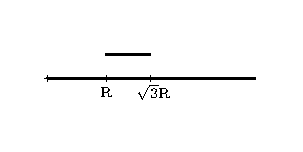
\includegraphics[width=.7\linewidth]{gfx/exhagon_barcode.pdf}
  \caption{Codice a barre persistente di $H_1$ per un esagono regolare di lato $R$}
  \label{fig:exhagonpersistence}
\end{figure}

Per chiarezza esplicitiamo il procedimento seguendo \cite{Curry}.
\begin{definition}[Persistenza di una nube di punti]
  Il processo di persistenza di una nube di punti è l'insieme delle seguenti operazioni.
  \begin{enumerate}
    \item Sia $X$ una nube di punti, cioé un sottinsieme finito di $\R^n$.
    \item A partire da $X$ si costruisce una famiglia crescente di complessi simpliciali (astratti) $\{X_r\}$ (ad esempio con il complesso di Vietoris-Rips) la cui omologia $H_q$ produce per ogni $q\geq 0$ uno spazio vettoriale persistente:
    \begin{equation*}
      H_q(X_{r_0}) \to H_q(X_{r_1})\to H_q(X_{r_2})\to \cdots
    \end{equation*}
    \item Il \Cref{thm:persistentdecomposition} fornisce un multi insieme di intervalli, che può essere visualizzato come codice a barre persistente.
  \end{enumerate}
\end{definition}

Utilizzando i codici a barre persistenti si riescono a individuare buchi $n$-dimensionali e a tracciarne l'evoluzione su più scale, o più in generale si possono distinguere due nubi di punti sulla base di proprietà omologiche dei complessi persistenti associati. Nel \cref{cap:esempi} mostreremo come è possibile utilizzare l'omologia persistente per fare questo tipo di analisi.

\section{Persistenza funzionale}\label{sec:functionalpersistence}

Nella \cref{sec:persistenthomology} si è visto come calcolare l'omologia persistente di una nube di punti, tuttavia non tutte le forme di enteresse vengono evidenziate dai codici a barre persistenti in questo modo. Si consideri ad esempio la \cref{fig:threeflares} in cui sono presenti tre rami che si distaccano da un nucleo centrale.

\begin{figure}[ht]
  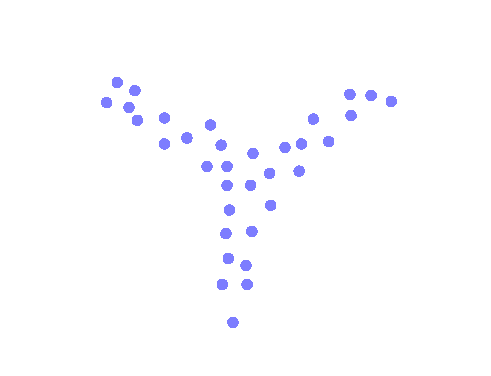
\includegraphics[width=.7\linewidth]{gfx/functional_all.pdf}
  \caption{Esempio di dati disposti in rami}
  \label{fig:threeflares}
\end{figure}

\`E possibile costruire un complesso simpliciale persistente la cui omologia evidenzi questa ramificazione? La risposta è fortunatamente positiva. Di seguito mostreremo la procedura più generale detta persistenza funtoriale, e vedremo come il caso in esame segue come suo caso particolare.

Sia $f:X\to \R$ una funzione reale definita su uno spazio metrico finito $X$. Allora per ogni $r\in \R$ possiamo considerare le preimmagini $X_r=f^{\shortleftarrow}([-\infty,r])$. Fissato un parametro $0<\rho\in \R$ una filtrazione di complessi di Vietoris-Rips
\begin{equation*}
  VR(X_{r_0},\rho)\into VR(X_{r_1},\rho)\into VR(X_{r_2},\rho)\into \cdots
\end{equation*}
e, applicando $H_q(-)$ a questi complessi, si ottiene lo spazio vettoriale persistente
\begin{equation*}
  H_q(VR(X_{r_0},\rho))\to H_q(VR(X_{r_1},\rho))\to H_q(VR(X_{r_2},\rho))\to \cdots
\end{equation*}

Infine, anche in questo caso il \cref{thm:persistentdecomposition} ci consente di costruire un codice a barre persistente.

Per rendere la persistenza funzionale sensibile a forme come quella in \cref{fig:threeflares} si può usare una funzione che misuri l'eccentricità di un punto $x\in X$ come
\begin{equation*}
  e_p(x) = \big(\sum_{y\in X} d(x,y)^p\big)^{\frac{1}{p}}
\end{equation*}
o, in caso $p=\infty$, $e_\infty(x) = \max_{y\in X}d(x,y)$. Poiché queste funzioni assumono valori alti per punti distanti dal "centro", prendiamo la rinormalizzazione
\begin{equation*}
  \hat{e}_p(x) = \frac{e_p^{max} - e_p(x)}{e_p^{max} - e_p^{min}}
\end{equation*}
che assume valori in $[0,1]$ e raggiunge entrambi gli estremi. Inoltre i punti distanti dal centro adesso hanno valori bassi, come si può vedere in \cref{fig:threeflarescomparison}.

\begin{figure}[ht]
  \begin{center}
    \begin{subfigure}[b]{.3\textwidth}
      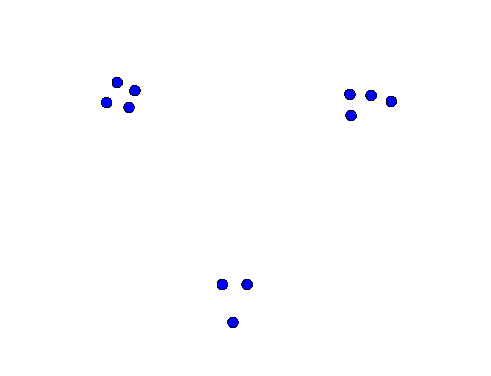
\includegraphics[width=\textwidth]{gfx/functional_small.pdf}
    \end{subfigure}
    \begin{subfigure}[b]{.3\textwidth}
      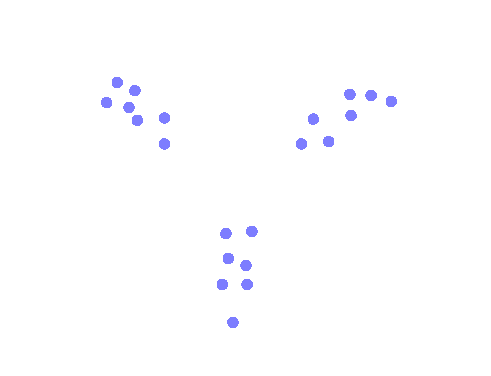
\includegraphics[width=\textwidth]{gfx/functional_medium.pdf}
    \end{subfigure}
    \begin{subfigure}[b]{.3\textwidth}
      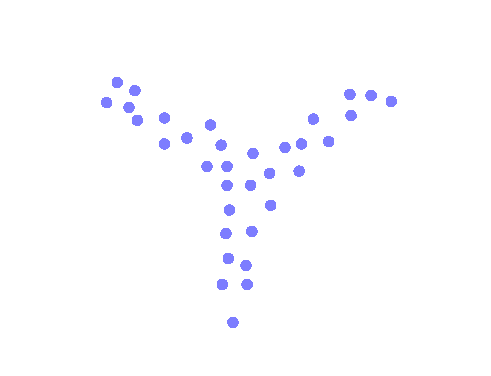
\includegraphics[width=\textwidth]{gfx/functional_all.pdf}
    \end{subfigure}
    \caption{$X_r$ al variare di $r\in [0,1]$}  \label{fig:threeflarescomparison}
  \end{center}
\end{figure}

Il codice a barre persistente corrispondente è mostrato in \cref{fig:threeflarepersistence}.

\begin{figure}[ht]
  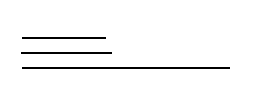
\includegraphics[width=.7\linewidth]{gfx/barcode_flares.pdf}
  \caption{Persistenza funzionale}
  \label{fig:threeflarepersistence}
\end{figure}

\section{Persistenza multidimensionale}

Nell'ultimo esempio nella \cref{sec:functionalpersistence} si può notare che abbiamo costruito una filtrazione di complessi simpliciali $(VR(X_r,\rho), \phi)$ al variare di $r\in [0,1]$, mantenendo però $\rho$ costante.

Tuttavia, sarebbe altrettanto valido fissare un parametro $r$ e costruire la filtrazione al variare di $\rho$ e calcolare l'omologia di questa. Più in generale, data qualunque funzione $f:X\to \R$ è possibile considerare le filtrazioni $VR(f^\shortleftarrow(-\infty,r],\rho)$ per valori fissati di $r$ o $\rho$ e calcolare il codice a barre persistente, tuttavia questo processo va contro il motivo iniziale per cui era stata introdotta l'omologia persistente: evitare di scegliere la scala di grandezza.

Si osservi che se $r<s$ e $\rho<\sigma$, allora
$VR(f^\shortleftarrow(-\infty,r],\rho)\into VR(f^\shortleftarrow(-\infty,s],\sigma)$ induce
una mappa $H_q(VR(f^\shortleftarrow(-\infty,r],\rho))\to H_q(VR(f^\shortleftarrow(-\infty,s],\sigma))$, quindi abbiamo a che fare essenzialmente con una filtrazione a più parametri, detta \emph{multifiltrazione} (vd. \cref{def:multifiltration}). Lo studio dell'omologia di una multifiltrazione è detto \emph{persistenza multidimensionale} di cui mostreremo brevemente i principali risultati seguendo \cite{Carlsson2009a}.
Anticipiamo già che non è possibile trovare risultati come il \Cref{thm:persistentdecomposition} che garantiscono l'esistenza di invarianti completi.

L'oggetto di studio della persistenza multidimensionale sono i moduli persistenti indicizzati da un insieme con un ordine quasi-parziale.\footnote{Si confronti con \cref{def:persistentset}, dove l'insieme degli indici è totalmente ordinato, $\R$}

Dati $u,v\in\N^n$, diciamo che $u\lesssim v$ se $u_i \leq v_i$ per ogni $1\leq i\leq n$.

Un \emph{monomio} in $x_1,\dots,x_n$ è un prodotto della forma
\begin{equation*}
  x_1^{v_1}\cdot x_2^{v_2} \cdots x_n^{v_n}
\end{equation*}
con $v_i\in\N$, che denoteremo $x^v$ con $v=(v_1,\dots,v_n)\in\N^n)$. Un \emph{polinomio} in $x_1,\dots,x_n$ a coefficienti in un campo $k$ è una combinazione lineare finita $\sum_v \alpha_v x^v$ con $\alpha_v\in k$. L'insieme di questi polinomi è indicato con $k[x_1,\dots,x_n]$ ed ha un'ovvia struttura di anello.

Un \emph{anello $n$-graduato} è un anello $R$ con una decomposizione in gruppi abeliani $R\cong \oplus_v R_v$, $v\in\N^n$ tale che $R_u\cdot R_v\subseteq R_{u+v}$. L'anello dei polinomi $A_n = k[x_1,\dots,x_n]$ è un anello $n$-graduato da
$k[x_1,\dots,x_n]\cong \oplus_v A_v$ dove $A_v= kx^v$, $v\in\N^n$.

Un \emph{modulo $n$-graduato} su un anello $n$-graduato $R$ è un $R$-modulo $M$ insieme a una decomposizione $M \cong \oplus_v M_v$, $v\in\N^n$ tale che $R_u\cdot M_v \subseteq M_{u+v}$.

\begin{definition}\label{def:multifiltration}
  Dato uno spazio $X$, una \emph{multifiltrazione} $\{X_v\}_{v\in\N^n}$ è una collezione di sottinsiemi $X_v\subseteq X$ tali che $X_u\subseteq X_v$ per ogni $u\lesssim v$ e tali che il diagramma
  \begin{equation*}
  \begin{tikzcd}
    X_u\arrow{r}\arrow{d}& X_{v_1}\arrow{d}\\
    X_{v_2}\arrow{r}& X_w
  \end{tikzcd}
  \end{equation*}
  commuta per ogni $u\lesssim v_1,v_2\lesssim w$.
\end{definition}
I complessi di Vietoris-Rips $VR(f^\shortleftarrow(-\infty,r_i],\rho_j)$ dalla \cref{sec:functionalpersistence} sono un esempio di multifiltrazione.

\begin{definition}
  Un \emph{modulo persistente} $M$ è una famiglia di $k$-moduli $\{M_v\}_{v\in\N^n}$ insieme con morfismi di moduli $f_{v,u}:M_u\to M_v$ per tutti gli $u\lesssim v$ e tali che $f_{w,v}\circ f_{v,u}=f_{w,u}$ ogniqualvolta $u\lesssim v\lesssim w$.
\end{definition}

L'omologia di una multifiltrazione di complessi simpliciali è un modulo persistente. Ad ogni modulo persistente può essere associata una struttura di modulo $n$-graduato nel seguente modo:

\begin{definition}\label{def:correspondence}
  Dato un modulo persistente $M$, definiamo il seguente modulo $n$-graduato su $A_n=k[x_1,\dots,x_n]$
  \begin{equation*}
    \alpha(M) = \bigoplus_v M_v,
  \end{equation*}
  dove la struttura di $k$-modulo è data dalla somma diretta e $x^{v-u}:M_u \to M_v$ è $f_{u,v}$ ogniqualvolta $u\lesssim v$.
\end{definition}

Il \cite[Teorema~1]{Carlsson2009a}, che riportiamo di seguito, ci dice che questa assegnazione è un'equivalenza di categorie.

\begin{theorem}
  La corrispondenza $\alpha$ nella \cref{def:correspondence} è un'equivalenza di categorie fra la categoria dei moduli persistenti finiti su $k$ e la categoria dei moduli $n$-graduati finitamente generati su $A_n = k[x_1,\dots,x_n]$.
\end{theorem}

Quindi il problema della classificazione dei moduli persistenti si riconduce alla classificazione dei moduli $n$-graduati finitamente generati. Tuttavia i moduli $n$-graduati con $n>1$ sono sostanzialmente differenti dal caso $n=1$ della persistenza omologica, in particolare Carlsson e Zomorodian dimostrano sempre in \cite{Carlsson2009a} che non esiste un invariante completo, discreto e indipendente da $k$ che classifichi i moduli $n$-graduati.

Quello che si può trovare è un invariante parziale che sia discreto e indipendente da $k$, detto invariante di rango che definiamo di seguito.

\begin{definition}
  Sia $\dot{\N}=\N\cup\{\infty\}$. Sia $\D^n \subset \N^n\prod \dot{\N}^n$ la sovradiagonale, cioé $\D^n = \{(u,v)| u\in \N^n, v\in \dot{\N}^n,u\lesssim v\}$. Per $(u,v), (u',v')\in\D^n$ definiamo $(u,v)\preceq (u',v')$ se $u\lesssim u'$ e $v\lesssim v'$.
\end{definition}

\begin{definition}[Invariante di rango $\rho_M$]
  Se $M$ è un $A_n$-modulo $n$-graduato finitamente generato, definiamo $\rho_M:\D^n\to \N$ la mappa $\rho_M(u,v)=rank(x^{v-u}:M_u\to M_v)$.
\end{definition}

\begin{rmk}
  $\rho_M$ rispetta l'ordine dato da $\preceq$, cioé se $(u,v)\preceq (u',v')$, allora $\rho_M(u,v)\leq \rho_M(u',v')$.
\end{rmk}

Nel caso di una multifiltrazione di complessi simpliciali possiamo dare una definizione dell'invariante di rango direttamente in termini dei complessi.

\begin{definition}
  Se $X=\{X_v\}_{v\in\N^n}$ è una multifiltrazione di complessi simpliciali, l'invariante di rango di $H_i(X_v,k)$ si può scrivere come
  \begin{equation*}
    \rho_{X,i}(u,v) = rank(H_i(X_u,k)\to H_i(X_v,k))
  \end{equation*}
\end{definition}

L'invariante di rango si restringe a un invariante completo nel caso di moduli $1$-graduati, tuttavia anche nel caso di moduli $n$-graduati può essere utilizzato per trovare proprietà topologiche persistenti cercando punti $(u,v)\in \D^n$ che sia lontani dalla diagonale. La lontananza dalla diagonale significa che la proprietà è persistente, ed è l'equivalente di cercare barre lunghe nell'omologia persistente.
